\documentclass[12pt]{article}
\usepackage[utf8]{inputenc}
\usepackage[a4paper,margin=1in]{geometry}
\usepackage{amsmath,amssymb}
\usepackage{enumitem}
\usepackage{parskip}
\usepackage{hyperref}
\usepackage{xcolor}
\usepackage{fancyhdr}
\usepackage{tikz}
\usepackage{graphicx}
\usepackage{eso-pic}
\usepackage{titlesec}
\usepackage{pdfpages}

\graphicspath{{../}}

\definecolor{kcpc-bg}{RGB}{250,250,250}
\definecolor{kcpc-text}{RGB}{20,20,20}
\definecolor{kcpc-muted}{RGB}{90,90,90}
\definecolor{kcpc-red}{RGB}{176,0,0}

\newcommand{\kcpcwordmark}{\raisebox{-0.15\height}{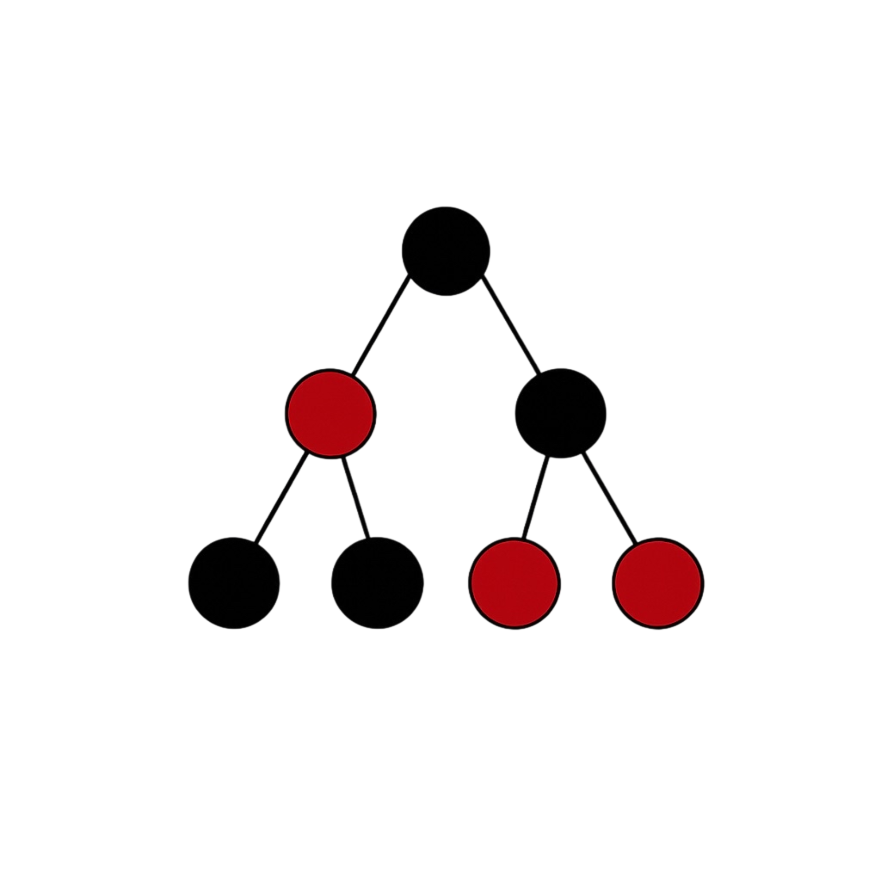
\includegraphics[height=0.55cm]{kcpc-logo.png}}}

\pagestyle{fancy}
\fancyhf{}
\lhead{\textcolor{kcpc-text}{\small\bfseries Problems}}
\rhead{\textcolor{kcpc-muted}{\small Hacking Session 1}}
\cfoot{\textcolor{kcpc-muted}{\small KCPC}}
\renewcommand{\headrulewidth}{0.4pt}
\renewcommand{\headrule}{\hbox
to\headwidth{\color{kcpc-red}\leaders\hrule height \headrulewidth\hfill}}
\renewcommand{\footrulewidth}{0pt}
\setlength{\headheight}{28pt}

\AddToShipoutPictureBG*{%
    \begin{tikzpicture}[remember picture,overlay]
        \node[opacity=0.035, at=(current page.center)]
        {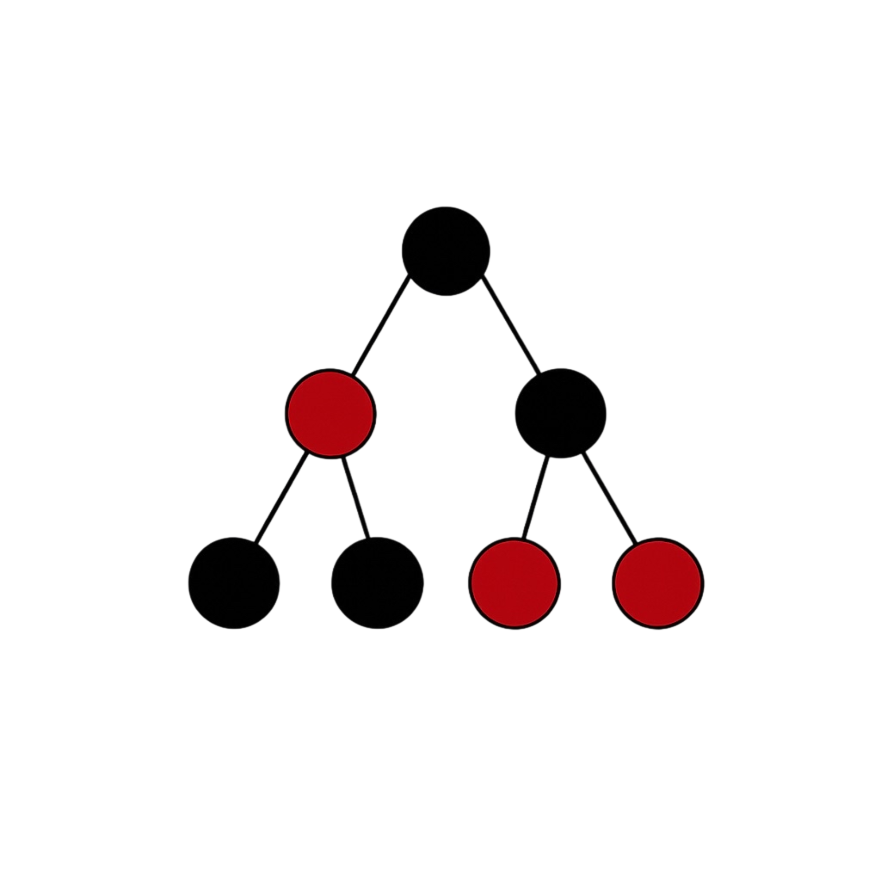
\includegraphics[width=0.38\paperwidth]{kcpc-logo.png}};
    \end{tikzpicture}%
}

\titleformat{\section}{\large\bfseries\color{kcpc-red}}{\thesection}{1em}{}

\setlist[itemize]{noitemsep, topsep=4pt}
\setlist[enumerate]{topsep=4pt}

\title{KCPC Hacking Session 1 Problems\\UKIEPC 2026}
\author{}
\date{}

\begin{document}
\maketitle
\thispagestyle{fancy}

\section*{Introduction}
\noindent
\textbf{Date:} 21 October 2026\\
\textbf{Contest:} United Kingdom and Ireland Programming Contest 2026\\
\textbf{Problems:} A-M (13 problems)

\medskip
The 13 UKIEPC 2026 problems cover a broad mix of topics, including letter substitutions, cryptarithms,
geometry, ratios, parsing, number theory, graph constructions, dynamic programming, and optimisation.
They range from approachable counting and modelling tasks to more involved algorithmic challenges, and
are not ordered by difficulty. This sheet accompanies KCPC Year 2 Hacking Session 1 on 21 October 2026;
the official contest booklet follows unchanged.

\clearpage
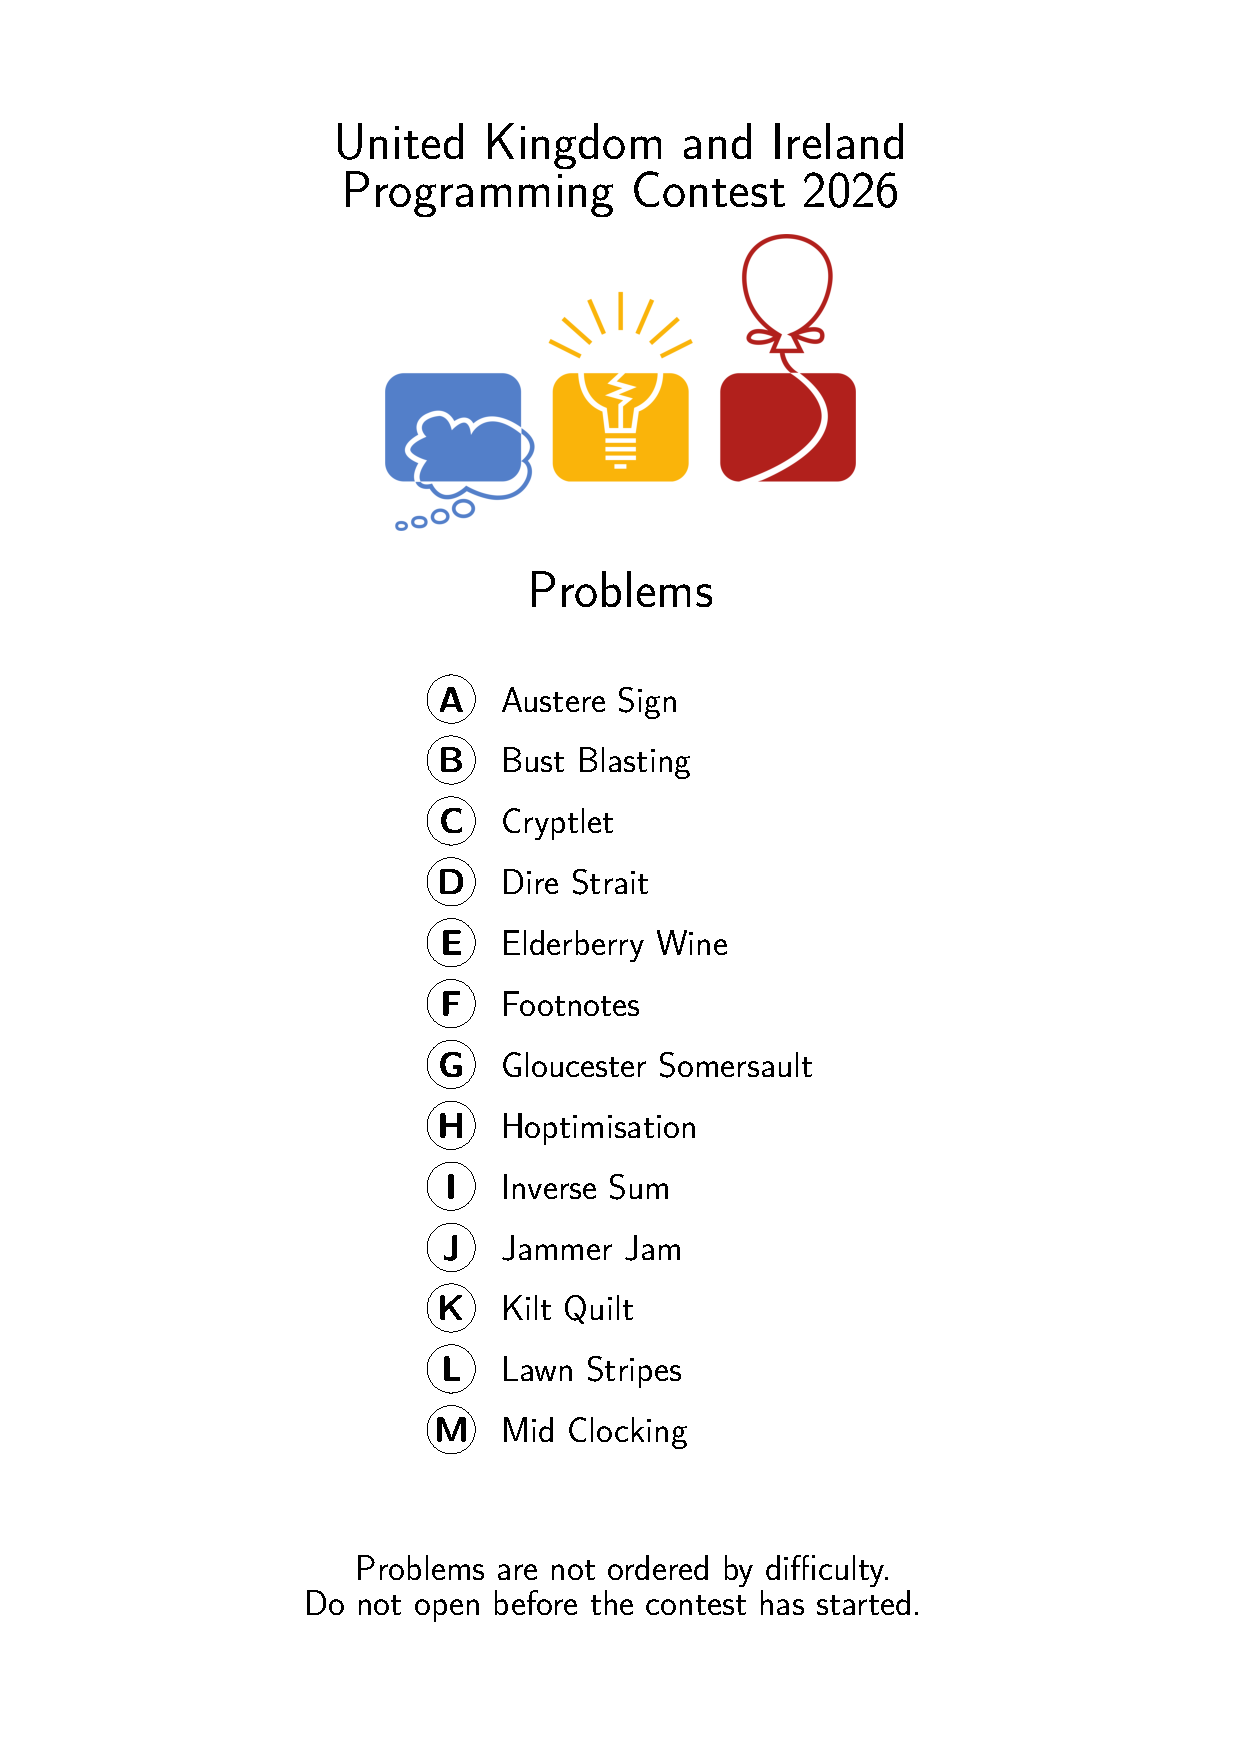
\includepdf[pages=-]{UKIEPC 2026 Problems.pdf}

\end{document}
